\section{Resultados}
\subsection{Las Redes como un Filtro}
\begin{itemize}
    \item Bode Diagrams
\end{itemize}
\subsection{¿Que Hace la Defensa JPEG?}
\begin{itemize}
    \item Intuition: JPEG removes noise that humans can't see
    \item Show graphs of jpeg defense vs epsilon of each attack
    \begin{figure}[h]
        \centering
        \begin{subfigure}[b]{0.49\textwidth}
            \centering
            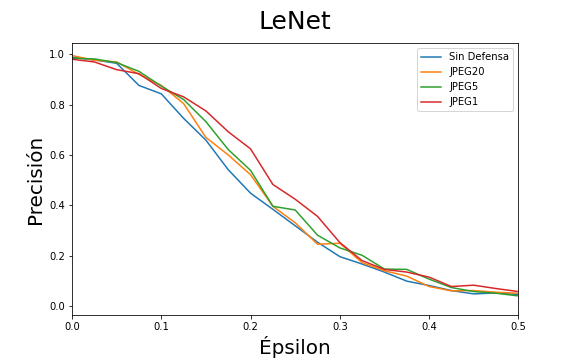
\includegraphics[width=\textwidth]{images/jpegdefense_vs_epsilon.png}
            \caption{LeNet}
            \label{jpeg_def}
        \end{subfigure}
        \begin{subfigure}[b]{0.49\textwidth}
            \centering
            % \includegraphics[width=\textwidth]{}
            \caption{ResNet (coming soon)}
            \label{jpeg_def}
        \end{subfigure}
        \caption{jpeg defense}
    \end{figure}
    \item bode diagrams with jpeg conversion as first layer
\end{itemize}
\subsection{Los Efectos de Overfitting y Overparameterization}
\begin{itemize}
    \item here they suggest overparameterization contributes to sharp gradient landscape \cite{ma2020understanding}...we find the opposite
    \begin{figure}[h]
        \centering
        \begin{subfigure}[b]{0.49\textwidth}
            \centering
            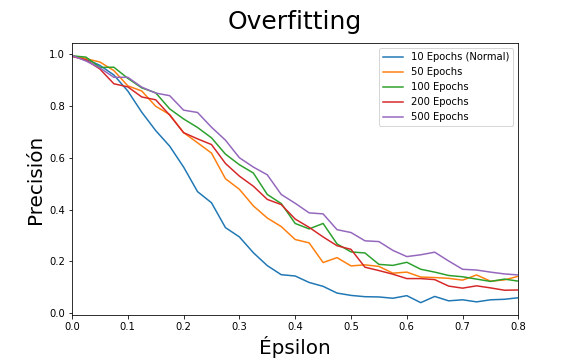
\includegraphics[width=\textwidth]{images/overfit_vs_attack.png}
            \caption{overfitting}
            \label{overfit}
        \end{subfigure}
        \begin{subfigure}[b]{0.49\textwidth}
            \centering
            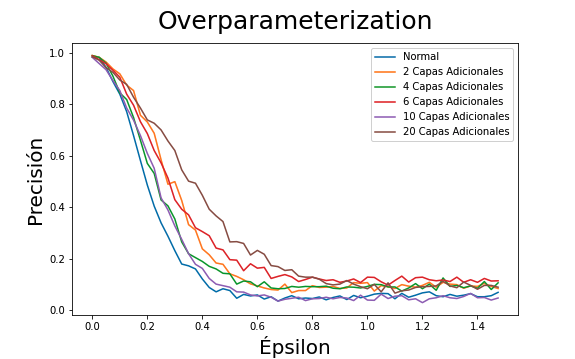
\includegraphics[width=\textwidth]{images/overparam_vs_attack.png}
            \caption{overparameterization}
            \label{overparam}
        \end{subfigure}
        \caption{Efectos}
        \label{overaparam_overfit}
    \end{figure}
    
    En la Figura \ref{overfit} se observa que conforme aumentamos el número de épocas (epochs), la precisión (accuracy) aumenta con respecto a cada épsilon, excepto para 200 épocas, cuya precisión es menor que la de 100 épocas, e incluso menor que la de 50 épocas para épsilon $>$ 0.5. Aumentar el número de épocas implica un sobreajuste (overfitting) de la red neuronal, lo cual significa que...
    
    En la figura \ref{overparam} se observa que conforme aumentamos el número de capas (layers), la precisión aumenta, excepto para 4 y 10 capas adicionales. Nótese que para épsilon $>$ 0.8, la red con 6 capas adicionales tuvo el mejor desempeño. Aumentar el número de capas implica una sobreparametrización (overparameterization) de la red neuronal, lo cual significa que...
    
    \item fix a large overparameterization and see if overfitting has the same effect
    \item pick an overparameterization and overfitting and check jpeg

\end{itemize}
\subsection{Saliency}
\begin{itemize}
    \item show figures from notebook of how adversarial noise attacks parts of the image that seem vulnerable (for example changing a 3$\to$8)
    \item Show Gradient-based localization of both imiage sets and how they change after adding adversarial noise\cite{Selvaraju_2019}
\end{itemize}
